
\documentclass[12pt]{report}
\usepackage{geometry}
\geometry{a4paper}
\usepackage{chicago}
\usepackage{makeidx}
\usepackage{tabularx}
\usepackage{graphicx}
\usepackage{color}
\usepackage{pdfpages}

\def\keywords{\vspace{.5em}
{\textbf{Keywords} \linebreak \,\relax%
}}
\def\endkeywords{\par}


\begin{document}
\begin{titlepage}
\begin{center}

% Upper part of the page. The '~' is needed because \\
% only works if a paragraph has started.
\textbf{\LARGE The University of Birmingham}\\[0.35cm]
\textbf{\LARGE School of Computer Science}\\[0.35cm]
\textbf{\LARGE MSc in Advanced Computer Science}\\[2.5cm]

\textsc{\Large First semester mini-project}\\[2.5cm]

% Title

{ \huge \bfseries Location Based Context-Aware Systems \\[1cm] }

{\large \textbf{Karthikeya Udupa Kuppar Manjunath}\\[1cm]}

\large{Supervisor: R Beale}
% Author and supervisor


\vfill

% Bottom of the page
{\large January 2014}

\end{center}
\end{titlepage}

\begin{abstract}
Technology has changed our lives over the years, computational power has increased drastically whereas hardware size has reduced, enabling us to design systems not only to solve the problem for us but also make our lives much more easier. The report focuses on one such technology, location-awareness. We try to explore the very roots of location-awareness, which is \textit{context} and awareness of context by understanding what context means, how it is categorised, its significance to the user and how to use it to improve user experience. We look into location, one of the most vital context and the basis of location-aware systems. We analyse the importance of location and look into the various ways to obtain location in detail under various circumstances and for various purposes and try to analyse which to use when building a system. We also look into the challenges in storing context information and how location information can be effectively stored and utilised between systems. Although there are various reviews done on context-aware application, we take a more modern approach by analysing two popular context-aware application in the consumer market and try to understand the various ways in which they harness location-awareness. The report also tries to analyse what are shortcoming in the present location-aware systems and what can be done to resolve it.

Based on the findings we design a prototype for a location based context aware system which would provide the user with personalised calendar with additional information in relation to the location information. The prototype tries to utilise the findings of the report to make the overall design more viable and useful.
\linebreak\linebreak\linebreak\linebreak
\begin{center}
\begin{keywords}
Location, Context, Context-awareness, Location-awareness, Ubiquitous Computing, Human Computer Interaction
\end{keywords}
\end{center}
\end{abstract}


\tableofcontents
\listoffigures
\listoftables
\newpage

\chapter{Introduction}
\noindent
In our daily lives, we always try to understand the scenarios and then come up with actions that we need to take to solve them. This process of understanding the current context is a subtle yet a very vital component of human existence. Knowing about the present context has always made our discussions more meaningful and performing day to day tasks relatively easy. Understanding of context and being aware about the surrounding conditions, although is a naturally existent and default behaviour of human mind, systems designed to assist us in performing various actions are not yet at the capacity to understand it completely.

The users of modern day are no longer restricted to a fixed workstation in a fixed environment anymore, with the advent of modern technologies computational power has increased and machine sizes have shrinker considerably. This along with availability of wireless access to fast network connections has lead to usage of diverse set of devices in a varied environment providing access to information almost seamlessly, whether be personal or professional or access to other publicly available resources. This has brought revolution both in the lives of the user and in the way systems are being developed. Weiser in his visionary article \cite{weiser1991computer}, described this as \textit{Ubiquitous computing}, ambient systems which would be weave themselves into our lives, rendering themselves invisible and catering to the informational needs of the user anywhere at all times. Although it is not yet widespread but systems are being designed to work based on the state of the user, making use of information about the user, his location, and other factors about the environment surrounding him being provided by the various sensors, information which is referred to as \textit{context}.


From all the available context information the relevant information is determined by the system and appropriate actions are taken. These context aware systems make the interaction with the system easier by providing customised information by understanding the user's need automatically. Increasing the amount of information would improve the performance of the system, this can be achieved by asking the user to explicitly provide the information, however this would not only be tedious for the user but also impossible as he might not know the relevance of the information himself. Also will defy the goal of context-aware system which is to improve the usability of system. Allowing the information's relevance to be decided by the system, would in-turn place the developer in the role of making decision about the significance of the information and the relevant action that has to be taken.

A vital aspect of the context comes from its dynamic and mobile nature, which is based on the awareness of location. It is one of the most widely used context information as its both resourceful and easy (compared to others) to obtain. The degree to which location is coupled with the system entirely depends on the design and actual function of the system. The location-awareness of the system provides it the ability to take actions automatically based on the user's present location hence improving the usability of the system further and reducing the efforts that the user has to put in order to obtain data. Location is also important as to obtain other significant information about the user.


Effective implementation of the context in the system is vital to make it more useful and friendly for the user. To make it possible it is essential to have an understanding of context and its possible usage, not only will it enable the developer in identifying the key contexts for their system but also help them in designing the appropriate context-aware behaviours.

\noindent

\section{Context}
A clear understanding of what context means is essential when designing systems based on it. Knowing significance of the information that is available and understanding of what constitutes as context for the user is the key to design effective systems. In general terms, context is \textit{``the circumstances that form the setting for an event, statement, or idea, and in terms of which it can be fully understood''} as defined by Oxford dictionary, however it can cover a much more in relation to computer systems being context-aware. 

There have been significant efforts made in order to aptly describe context and what it means to be be context-aware. The earliest definition is from \cite{schilit1994context} who introduced this term, he defines context-aware as the user's current location from where the system is being used, information about the people, devices and other objects situated in the vicinity and any information regarding the changes to these entities. Additional parameters such as day, time, temperature were also been considered vital \cite{brown1996supporting}. \cite{prekop2003activities} defines it as any state of the environment which is significant to the user and in which the application reacts or and an event occurs. 


The definitions clearly indicate a need to include the environment of the user which is known to be changing constantly, it not only includes the user's surroundings but also his social conditions, physical state as well as the available computing resources at hand. Which is all very essential, as the context has to be related to the condition of the application along with the user's using it.


The most relevant definition for context is by \cite{dey2001understanding} which specifies that context refers to any information which can be used to represent the present state of the entity which is relevant to the interaction between the user and the application. The relevant entity can be anything which provides information about the user either implicitly or explicitly. He rather weighs on the context that is being provided rather then the way it is done. 


\textit{``Context is any information that can be used to characterise the situation of an entity. An entity is a person, place, or object that is considered relevant to the interaction between a user and an application, including the user and applications themselves.''} - \cite{dey2001understanding}


It is also vital that the definition of context specifies the context based on present situation and does not identify context in general, as context with relation to the application and the user can be very specific from what context constitutes of in general. For example, if the user is driving a car then traffic information is relevant and hence it is contextual information, however if he is waiting for a train, traffic would not hold any relevance and hence would not be a context. Thus, definition of the context has to be governed by the current situation of the user and the application.

\section{Categorisation of Context}

It is very essential while designing of context aware systems to identify the information that is relevant to the user's current state and classification of context certainly helps in this by enabling the system designers to identify the requirement for their application.

Various methods have been proposed to classify the context features over the time. For instance, they can be broadly classified as external and internal \cite{gustavsen2002condor}. External refers to quantifiable parameters obtained using hardware sensors such as a GPS receiver whereas internal refers to user generated content such as user's calendar schedule, his travel plans etc. \cite{chen2000survey} classifies context as active and passive, wherein the first type refers to the ones which actively play a part in the working of the application visibly whereas the second one refers to the ones that have no direct impact and are not as critical as their active counterparts. \cite{abowd1999towards} simplifies the characteristics of context based on several existing systems, each system is considered to have at least a few consistent contexts associated with entity, location (the position of the object, this can be relative and with relation to other objects), identity (refers to the unique identifier which is used to identify the entities), status (properties associated with the entity at the given time) and time (in order to sequence the event in the correct order).

\cite{schilit1994context} on a broader level classifies the context as follows.
\begin{itemize}
	\item \textit{Physical context} - Measurable physical factors such as movement, touch, sounds, temperature.
	\item \textit{User context} - Information about the user which is related to the user such as his location, his social and personal profile.
	\item \textit{Computing context} - connectivity to the network and hardware interfaces.
	\item \textit{Time context} - time is very vital as information is relevant at a given instance of time.
\end{itemize}

Additional parameters have been considered by \cite{chen2000survey} which are very essential, especially when considering the more modern devices which are personal and portable. All this contributes to the historical aspect to the context \cite{chen2000survey}, this is accumulated over time of usage of the application, this historical context can be used to adapt the system accordingly severing as another source of information.

\section{Context Awareness}
Awareness can be described as \textit{``the state of knowing about the environment in which you exist; about your surroundings, and the presence and activities of others''} \cite{wisneski1998ambient}. Context awareness is very much associated with this, as it refers to the awareness of the application to the present condition in which it is functioning. The earlier definitions were fairly simply, they refer to application that first detect and then react accordingly to the alterations that have occurred in the current environment or context \cite{schilit1994disseminating}. They were similarly dictated by the ability of the system to detect, interpret and react to the context. However with the advent of generic devices which can handle multiple application which can provide information to the user without actually having to the process of sensing and detection itself, hence context-awareness can be considered as an ability to adapt itself to the dynamic context of the user and the application. Dey's \cite{abowd1999towards} definition takes a more specific approach and restricting it to include only those devices that modify their behaviour based on the context change.

What we can conclude from these definitions is that the context-awareness focuses on the needs of the user and would always consist of three aspects automation, adaptation and personalisation \cite{nelson1998context} which are essential for any system to be considered as context aware.

\section {Role Of Context-Awareness in Improving User Experience}

The recent interest in context-awareness and context-aware application can be attributed to the fact that it holds enormous potential in creation solutions that would not only improve the user experience but also prove helpful in their daily lives. Needless to say, context forms a basis of all such systems which aim at showing ambient intelligence. The context is always altering, hence the need of the user or the information that is relevant to them also changes constantly. The context-aware systems hence consistently gather information about the present context of the user and provide him with information that suits his present need while requiring almost no user attention.


This holds the key to significantly improve the lives of the users. Providing them information at the right time, will save them valuable time, help them improve their efficiency and optimise their way of work and living. For example, if the user travels everyday to office at a certain time, providing him information about the traffic beforehand would help him choose a better driving route, presenting him with optimised and most viable travel option rather then his regular one would be even more effective use of context. The ability of context to interpret and use the user's information without distracting him from other important tasks also shows the vitality of context awareness in larger ubiquitous systems. 

\cite{moran2001introduction} suggests that the need for context-awareness arises to keep us secured from the unfortunate negative impact technology has in our day to day lives, thus by automating functionalities based on the condition we might be able to keep the user from going astray because of his need to use technology and keep us away from the control loop required to manage these systems \cite{erickson2002some}.

\chapter{Location Awareness}

Of all the context information available the most prominent and widely used is location. Although, compared to others location might seem very simple and basic, yet the role it plays in context-aware system is very vital. Location is an essential part of the present day systems especially due to the mobility factor in them, the improvements that can be done to the user experience with the location context are immense and very promising.

\section{Importance of Location \& Location Awareness}

Systems are no longer limited to bulky desktops inside offices, dynamic environment is a key concept in ubiquitous and modern day computing hence all new systems especially the mobile systems leverage from the location context. The importance of location can be established by the amount of research being done in the field of location sensing and location-aware applications in the last few decades. Even the earliest of context aware applications, Active-badge systems \cite{want1992active} was build to utilise the location context.


Location has been an integral part of various systems for a long time in the form of location services, which can are defined as \textit{``services that integrate a mobile device's location or position with other information so as to provide added value to a user''} \cite{schiller2004location}. However, location-aware services make use of the location of the user to adapt themselves accordingly, hence making location-aware a subset of location based systems. 


One of the factor in location emerging as a widely used context is the ease of obtaining location when compared to other. It can be obtained with fair amount of accuracy fairly easily and with not much usage of resources. But the key reason for its elevated status is the information that it can provide, both directly and as an index to lookup other related information \cite{schilit1995system}. It can also be used to infer other significant context such as temperature, traffic condition etc. It is a very efficient way to improve usability of the system to present the user with the information that he requires at that particular place hence minimising his need to interact with the system, hence saving his time and efforts \cite{kaasinen2003user}.


\section{Location}

Location usually indicates the position of an entity at any given time. However, there can be various variations in the nature of location and it depends on the designer to select the appropriate one based on the requirement of the system. In many cases, an absolute physical location is required, which is usually a spacial representation of the user in a 2D or 3D cartesian system \cite{rodden1998exploiting}, this is usually in reference to a fixed point in space, which can be anything from the centre of the earth or in the building the user is presently located in whereas in other cases we require a more relative location, for example if the user is inside a room or in the vicinity of a certain device which would require sensors at both ends, best example of which can be seen in the active badge location \cite{want1992active}. The granularity of the location information is also an essential aspect and depending on the accuracy needs of the system a proper location extraction technique has to be selected.


\subsection{Components Of Location}

Although there are various technologies with each having its own way of representation of the location, each of them do consist of some common and standard properties. \cite{schiller2004location} tries to identify the essential elements in the location information.

\begin{itemize}
\item \textbf{Cartesian Coordinate System} - The coordinate system represents the position in a 2D or 3D space. The most common and extensively used is the Latitude, Longitude and Altitude model. It considers the location of the entity in three dimensional space over the earth's ellipsoid surface. There are other systems that consider earth's centre of gravity as as the initial point and map the space above it, some consider mapping the coordinate over the earth considering it as a sphere or a cylinder.

\item \textbf{Accuracy} - Location sensing systems are not always accurate, there are always certain precision issues that have to be considered. Depending on the method that has been selected the accuracy varies. Even with the same method, accuracy can vary over a time period as it depends on various factors, such as weather, positioning of the satellites, signal strength etc. This can be observed by the variation of location over a period of time in mobile device even when it is in the same location. This has to be kept in mind while designing of systems that require accurate information, hence the precision has to be considered.

\item \textbf{Scope/Relative Area} - The scope of the location obtain depends entirely on the technique that was used to obtain the information. For example, the location obtained from the GPS system is valid worldwide (although a GPS location system would not work for systems in geosynchronous or planetary orbit, which would then have to use more complex systems such as Optical Navigation System \cite{rathbone1988optical}, which would increase the scope of the location), but a location obtained by an indoor system is only valid over a short area, usually in a building or a floor of a building and is relative to that system hence is a local location.


\item \textbf{Coverage} - Coverage refers to the area which the system is able to successfully map the entity's location in. This varies based on the type of service as well, GPS usually, would be able to sense the location of the user throughout the globe but an indoor location system has a very limited coverage and would not be able to locate the entity when out of that area.
\end{itemize}

Depending on the technique used and further that was applied to the location data, additional information can also be made available but require other elements in order to obtain it, such as speed, orientation etc.

\section {Location Sensing Technologies}
A prime component of any location aware system is the sensing technology that is to be used in order to determine the user location. The best and possibly the most accurate way to obtain information is to ask user about his present location, but that would involve the user having to interact with the system and having accurate information, hence location-awareness has to be automatically obtained and processed. Although a relatively easy context to obtain, sensing location is a complex process and involves various governing factor. Primarily it is the actual need of the application that decides the best technology to use but other factors such as accuracy, frequency of updates required, power consumption factors, coverage area and reception also play an vital role. A single technology will not be able to handle all the location identification problem of any location-aware system. Each have their merits and demerits. Based on the technology used to fetch the location we can broadly classify the systems into satellite based, Network based, Hybrid and indoor positing systems.

\subsection{Satellite Based Positing Systems}
These systems provide information about location, precision of which is fairly limited. They are usually absolute and provide location information as per a coordinate system. They usually depend on external known points in space to identify their location based on it. These points can be satellites or fixed base station on earth.

\subsubsection{GPS}
The GPS or Global positioning system is a one of the oldest of the location systems, introduced in the 1960's by US's Department of defence to meet the need for a satellite based location system. Originally known as Navigation System for Timing and Ranging (NAVSTAR) was restricted to the military but subsequently was opened for public usage \cite{ta2011global}. Consisting of 24 satellites in orbit around the earth in 6 different orbits. It provides a free-to-use one way communication mechanism in determining the location of the user. There are two services that can be availed through GPS satellites. \textit{Precise Positioning Service} (PPS), which is for the armed forces and provides a precession of 22m and there is \textit{Standard Positioning Service} (SPS) for civilian use providing precision of 100m \cite{schiller2004location}.
 
Each satellite constantly transmits its location in space at a given time, if the device consists of GPS receiver 
it would be able to pickup the signal, these signals are time-coded and synchronised to provide more accuracy. The signal from these satellite is then coded into 3D representation in space \cite{djuknic2001geolocation}. There are several advantages of using GPS mainly the positioning can be done, in principle, throughout the world. and also the fact that the location information can be obtained without no network requirement or additional equipment on the user's end \cite{djuknic2001geolocation}. But there are several downfalls.


\begin{itemize}
\item The system only works when there are sufficient number of satellites accessible to the user.

\item Performance of the system fails considerably in indoor and urban environments \cite{hazas2004location} And even in outdoors its accuracy can be considerably low at times.

\item Although minimal, environment conditions impact the the working of the system \cite{schiller2004location}. The working can also be effected in RF environments \cite{djuknic2001geolocation}.

\item A considerably amount of time is taken by the receivers to fetch location when initiated for the first time \cite{hazas2004location}.

\item The power requirement, cost and size of the receiver has also become a significant factor with constant reduction in the device sizes \cite{djuknic2001geolocation}.
\end{itemize}

There are other similar satellite systems which operate similarly to GPS. The Russian system, GLONASS (Globalnaya Navigationnaya Sputnikovaya Sistema) operates idenical to the American GPS. European union has also launched its initiative in 2006 called the GALILEO.


\subsubsection{DGPS}
DGPS or differential GPS uses the available information from the GPS information, however in order to provide a more accurate location it interacts with a stationary receiver known as the base receiver, which is on earth. Their location is fixed and and known with utmost precision. The device and the base receiver both obtain the position from the satellite however since the base receiver knows its exact location, it identifies the differentials and sends the correction information to the device \cite{roth2002mobile}, hence improving the accuracy up to 1-3m \cite{schiller2004location}. The system assumes that the device and the base station are in proximity as to receive single from the same satellite. 


\subsubsection{WAAS}

Wide area augmentation system is an extension of DGPS, it works in a similar way as DGPS, wherein the base receivers calculate the correction data, but instead of sending it directly to the user the information is sent to a central station known as the wide-area master station, which inturn calculates the correctional data for the whole area and passes it on to a geo-stationary satellite. This information is then provided to the device and appropriate corrections are done \cite{corrections2004comparing}. This provides an even more refined and precise location then DGPS. At present the WAAS is limited to America, however an European version of WAAS known as European Geostationary Navigation Overlay System or EGNOS was launched in 2009.


\subsection{Network Based Positing System}


One of the primary disadvantages of satellite based positing systems is the cost that is occurred in installing and maintaing them. The installation is not a one-time cost, as satellite have a limited lifespan and have to be replaced often. To reduce the pricing issue, systems utilising the existing wireless networks can be used to locate user/devices.

\subsubsection{GSM}
Global system for mobile is a system with wide coverage and easily accessible through any modern day mobile device. The system of cell towers already exist, hence using this system to obtain location can significantly reduce the cost of the overall process. Each user's cell tower access is registered in the database, based on it his location can be identified to a specific cell area \cite{schiller2004location}. The time to get a fix on location is very less since the connection is already there. Also, there is no need for additional hardware and there is no additional power consumptions as well \cite{djuknic2001geolocation}. However, the location information that is obtained is of far inferior quality then that obtained through satellite based systems. Also the location information being shared with the provider arises a serious privacy concern for the user which did not exist in the satellite based systems. Also, the dependency of obtaining a location fix is now on the network coverage which might not good everywhere when compared to GPS and other similar systems.


\subsubsection{Wireless LAN}
This system, initially implemented by Microsoft \cite{bahl1999user}, utilises the signal strength from the various WiFi access points to identify its location in space (size can vary from a building to couple of blocks). The location information obtained through this system is can be as much as 1 meter. The system is very efficient in providing location in urban environments and does not require any further hardware installation other then a WiFi receiver, which is usually present in modern day mobile devices and a mesh of wireless network. There is no dependency on the environmental factors such as weather as the signals are local and there is no dependency on remote satellites or cell towers. The system is however restricted by area and the density of wireless network available. Additionally it requires an initial training, either manually or through a virtual model of the area to function \cite{schiller2004location}.

\subsection{Hybrid Systems}

\subsubsection{AGPS}
Assisted-GPS uses both GPS and GSM to allow the device fetch a more precise location information. This system has several advantages over the traditional GPS systems \cite{djuknic2001geolocation}. The assistance server has information about the location of the satellite in the area and far more processing power then the device, it can provide the device with the satellite information hence reducing the search space hence reducing the time for first fix by a large factor. This also effects the power consumption of the device as it would require to be operational for a very short period of time. Since the system is depended on the base station, any improvement made on that end would benefit the user without having to make any further investments. The only downside to AGPS is the requirement of both GSM and GPS hardware modules and network connectivity to function.

\subsection{Indoor Positing Systems}

In modern cities, which are usually concrete jungles with tall skyscrapers and multi-level shopping complex and factories, location of the user obtained from either satellites (provided signals are available inside the buildings) or network does not meet the need, a more refined positing system is required. Indoor positing systems meet the specific need for obtaining position inside buildings. These systems usually provide relative position and have a very limited scope and coverage. 


\subsubsection{Infrared Beacons}
One of the earliest of the indoor positioning system, first seen in Active badge location \cite{want1992active}. The system utilises IR beacons provided to each user which emit IR pulses carrying specific code. These pulses are received by the sensors installed throughout the building which then transmits it to the main computer, hence being able to locate the location of the user in realtime anywhere in the building. The power consumption of the devices is minimal and so is the cost \cite{schiller2004location}. The technique however has its limitation, firstly it has a very strict and small coverage area, secondly there is no authentication in place, so anyone could send an identical signal and fake one's location. Also, infrared are unable to penetrate walls effectively hence required several receivers to cover the most possible area.


\subsubsection{Radio Beacons}
Radio Beacons unlike Infrared are able to penetrate walls, and with the help of multiple radio beacons location can be calculate. This is very similar to the satellite based positioning system. RFID (Radio frequency identification) transponder, which are also based on radio beacons, on the other hand do not have a power source, but use the energy from the incoming signal to either store or send data. They can be used to track an object's location by determining if the object was ever present in the vicinity of the transponder. RFID does not however provide any information about the exact location of the entity. More recently NFC (Near field communication) technology which is also based on radio signals has been introduced in mobile phones and is being considered as an alternative to RFID's and to provide location specific information to the user \cite{siira2009location}.


\subsubsection{Ultrasound Based Systems}
Systems equipped with ultrasound capabilities require the user to user the device to send a request to the server, which then activates a signal generator to generate an ultrasound signal which when received by the user's device is forwarded to the server. The server uses this information to calculate the position of the user. The location obtained through these systems are very precise.


\subsubsection{Video Based Systems}
Visual information is widely used by humans in day to day lives to locate user, but for a computer system to do the same can be very daunting. The processing required to handle visual information can be immense and for such a system to work, installation of cameras would be required which can be quite expensive. These systems relay on the ability of the system to detect colours and patterns in visuals. In an implementation experiment \cite{starner1997augmented}, visual tags were given to the user and cameras were installed in the premises. Considering the fixed nature of the patterns and camera, two cameras can be used to triangulate the exact location of the user and also identify him.

\section{Selecting the optimum sensing technology}

As it is clear, there are several ways to determine location, however as discussed earlier, the method to be used would highly depend 'on the nature of the location-awareness that the solution requires. For general purpose usage, GPS is the most recommended option, as it is cheap and comes installed in most of the modern devices hence making it very viable. It also provides a fairly accurate location output. Development of application for existing platforms such as mobile devices restricts the choice to a limited due to their fixed hardware, hence the designer have to make use of the hardware that they are provided with. More recent devices are equipped with GLONASS, AGPS and application which are developed for these platforms can leverage the technology. If the application does not require a very precise location (for example, weather application, which would require a city level accuracy), Network based positing systems would be more apt, as they do not consume any additional power and yet meet the need.


\begin{table}[htdp]

\begin{center}
\begin{tabularx}{\textwidth}{ XXX }
 
  \begin{center}\textbf{Method}\end{center} & \begin{center}\textbf{Precission}\end{center} \\
   \hline
  Global Positioning System  & 5m - 25m  \\
  DGPS   & 3m    \\
  WAAS   & 3m    \\ 
  GSM   & Cell's Area    \\ 
  WLAN    &  upto 2m (depends on waypoints) \\ 
  Infrared    & Coverage area of the transmitter/receiver \\ 
  Radio    &    Cell area \\ 
  Ultrasound    & 0.1m (depends on system's implementation)    \\ 
  Video    & Varies on the camera resolution \\ 
   \hline
  \end{tabularx}

\end{center}
\caption{Accuracy comparison of the various location sensing technologies.}
\label{accuracy comparison}
\end{table}%


RFID's and NFC's meet a very specific need, they are usually best suited where information has to be presented when a certain location has been reached. Although, it does not provide exact location information but can be used in various scenarios such as tourist guides, where the audio is played as soon as the user enters into a certain room or information is displayed on the device when brought close to tag near an exhibit.


Indoor location systems, even though have been existent for a considerable amount of time, but have not been very popular. In fact hardly any of them have reach a mass production state. If the system that has to be implemented requires a very precise location even within buildings and precision cannot be comprised with, indoor systems such as Ultrasonic or Infrared can be used. However, no single system has complete accessibility and a combination of multiple systems working together to provide a reliable and precise location would be the most recommended got any location aware system.

\chapter{Context Modelling}
\section{Challenges In Modelling Context}

Representation of the contextual information while being stored and processed is very essential for development of context-aware/ubiquitous systems. Context model can be defined as a pattern to represent an object's or an user's context \cite{zhang2011survey}. However we need to understand that context has a nature that is not very similar to the regular data that we tend to model in case of normal systems \cite{henricksen2002modeling}.

\begin{itemize}
\item \textit{Variation In Characteristics} - The context information is usually collected from a wide range of sources, some information is static in nature whereas some is sensed while some being provided by the user themselves and a major of part of it is deduced by the system, hence they are heterogeneous both in terms of quality and the persistence of the information \cite{henricksen2006developing}, sensed information is prone to have noise and also tends to change at a very frequent rate whereas the static information such as the name or date of birth of the user are to remain the same.
\item \textit{Imperfection} - Context if not representing the true state of the real world is considered as imperfect. Considering nature of dynamic context, information tends to change and hence context that might be true for a given timeframe might not be perfect once it has passed, provided it has not been updated.
\item \textit{Alternative Representation} - Information is being extracted from various sources, the sources might not have the exact representation as required by the systems. Hence an alternative representation is required. The model should be able to handle multiple abstraction of the same information and maintain a relation between them.
\item \textit{Inter-relation} - Context of one kind alone does not appear to be so important, however when associated with other contextual information there are various conclusions that can be made. Also, some context information might be associated in deriving other.
\end{itemize}


\section{Location Specific Context Model}

Due to various different types of location-sensing technologies, each technology has its own method of presenting location information. This creates a problem when we try to integrate location information further with more complex context, hence a unified location-aware model is required to allow an efficient integration of the components. The representation of information can be based on several base models to represent context the below mentioned are some models that are apt for usage of location-aware context.


\subsection{Key Value Context Model}
One of the simplest model to describe a context is to use key-value pairs to identify properties and their values which describe the context for the object. Due to its simple nature it was used widely in earlier systems. Although it is unable to represent complex contexts but can be used to efficiently represent information such as location and functionalities.

\subsection{Markup Context Model}
Markup type model where in the context is stored as markups in a hierarchal structure with attributes stored along with the context information. The information is shared through standard markup languages between application. An example of this in reference to location-awareness would be NeXus \cite{hohl1999next}, where the information is stored in Augment World Modelling Language, a derivative of XML, it contains geographical information in Geographical markup language(GML), this information is usually spatial instead of being absolute and can be queried through its own querying language. 


\subsection{Ontology Based Context Model}
Context of any type usually represents relationship to the user or object, making ontology an appropriate model to store context of any kind. Ontology based model rely on relationships in describing or inferring the the context.


Various location models use ontology based model to create a more specific model. One of the example is the semantic location-aware model \cite{li2008semantic}. The model focuses on geographical containment of spaces and accordingly maps it. The sub-spaces known as cell contain information about objects within its containment field and their relationship with each other. This also allows the regulation of policies and provides more control over the independent cell area.


\chapter{A Review Of Modern Location Aware Applications}

Location-awareness is one of the earliest harnessed context in the context-aware application. Nearly all early application's that were context-aware were build either solely on location or dependent heavily on it \cite{baldauf2007survey}. Over the course of many decades since the Active badge location \cite{want1992active} there have been considerably number of application that have been build to be context-aware, \cite{chen2000survey} covers a wide variety of such application and have been extensively analysed. However, we are going to look into two more modern applications that were developed for present day mobile devices that are widely used in day to day lives and exhibit location and context-awareness. 

\section{Google Now}
An artificially intelligent personal assistance application developed by Google specifically for mobile devices, Google Now \cite{google2014app} is an modern example of state of the art context-awareness implementation in the currently available mobile devices in the consumer market. The application launched in 2012 provides the user personalised information based on his personal profile and his present location.

The application connects to the user's google account accessing information from his email, calendar and search history among other things. Based on the information and his location the user is presented with customised set of information. The location here acts as an input, helping the application infer other context and fetch meaningful information based on it \cite{koubek2013augmented}. The information is displayed in the form of cards, with each card displaying one set of information. There are various ways in which the application showcases its location-awareness.

\begin{figure}[htbp]
 \centering
 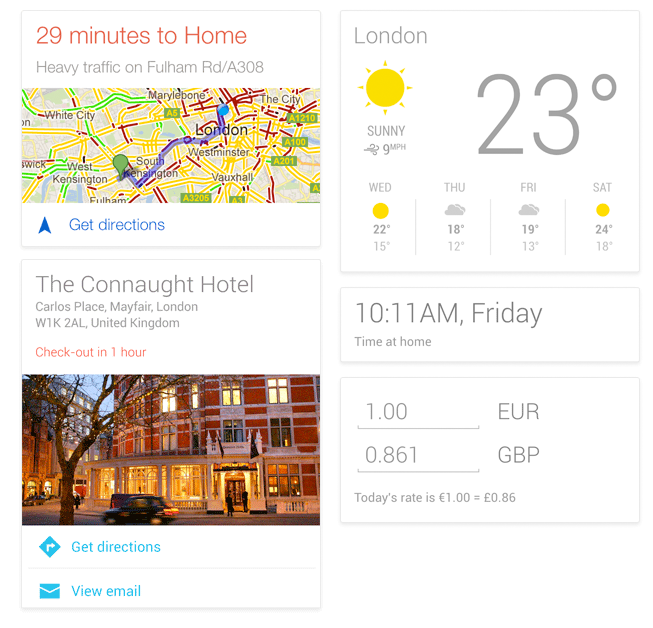
\includegraphics[width=90mm]{GoogleNow.png}
  \caption[Various Google Now \textit{cards} displaying information to the user.]{Various Google Now \textit{cards} displaying information to the user. (\textit{From the Google Now page - \cite{google2014app}}}
 \label{figure:GoogleNow}
\end{figure}

\begin{itemize}
\item \textit{Weather Information} - The application presents weather information based on the user's present location. If the user is presently not in his default region, the application considers he is travelling and weather information of both his present and his home address is displayed. Additionally, the application smartly switches between GPS and GSM/WLAN based location sensing.

\item \textit{Time Information} - If the user is in a different time zone other than his default one, time information for his default one is displayed.

\item \textit{Place Information} - The application monitors the user's location for places of interest and in case he is in a place with tourist attractions or there are other interesting events and places, they are displayed to the user. If the user is in a new location and there are certain indications in his email (e.g. hotel reservations) about the intended destination, the travel information to that location is shown automatically.

\item \textit{Transit} - For commuting, the application detects patterns of user's daily travels (for example home to office) and over the time it provides the user with scheduled information about the traffic on the preferred route. Additionally, the application tracks the user's mail and identifies any information corresponding to travel and in case of such findings, the travel information (for example flight timings) are shown to the user on the scheduled time.
\end{itemize}

Additional localised information includes providing of instant translation services to and fro from the native language of the new location, current conversations from the user's default currency to even providing information about possible places to take photo at the default location \cite{google2014app}.
 
The process of monitoring the information is almost invisible and takes almost no input from the user. The application uses tags to identify the location for the person such as his office, work place and other important venues.

\section{Siri}

Siri\cite{siri2014} is an Apple's alternative to Google Now. Siri is a voice based assistance integrated with artificial intelligence and uses location-awareness to provide the user information. Siri takes input from the user and combines with the current location of the user to perform actions. It's build specifically for Apple devices running iOS, Apple's proprietary operating system for mobile devices.

\begin{figure}[htbp]
 \centering
 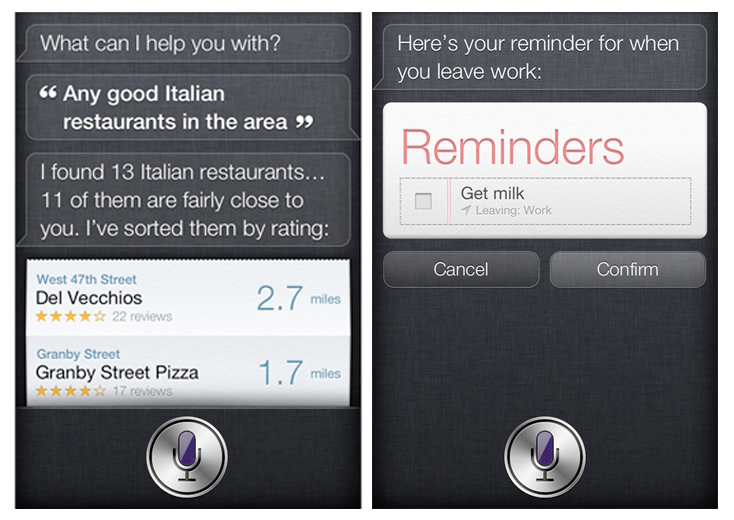
\includegraphics[width=90mm]{Siri.png}
  \caption[Interaction between the user and Siri.]{Interaction between the user and Siri, notice the absence of any absolute location information in the queries.}
 \label{figure:Siri}
\end{figure}

\begin{itemize}
\item \textit{Location Specific Search} - Siri enables users to put in queries vocally, which then is processed through natural language processing. The query is then associated with user's present location to search geo-fenced information. For example, the user may query about nearest italian restaurant, it would search for italian restaurant in the database within the particular range of user's location. Due to its interfacing with a natural language processing engine, it can perform various such queries, like finding distance to a particular place, or driving directions, or finding the nearest gas station.

\item \textit{Location Tagging \& Location Triggered Events} - Various locations in the phone can be used in the form of tags. Which can be used to trigger event when the user is at that location. For example, the user can create a reminder to call his boss when he gets home. The application, recognises the user's contact details and relates the word "Home" to the home address of the user and creates a location specific trigger. This reminder is triggered when the user reaches the specific location. The triggers also works when the user leaves his particular location.

\end{itemize}

\chapter{Issues}

As we have seen the possible use of location awareness especially with emergence of mobility and handheld devices is immense, already it has proven to be extremely useful the existing applications. However, as any developing technology, location-awareness has its own concerning issues and challenges which would have to be seen to before a large scale adaptation of the technology.

\section{Privacy}
Of all the concerns of location-awareness, the one which is taken most seriously is location privacy. The very concept of location-awareness requires the user's location to be known to the system and in most of the cases without asking him about it. knowledge of the location of a person can be used to do various ways for wrong tasks which can range anywhere between business sending the users provide localised spam to use of location information to infer other personal information about the user such as his schedule, health conditions, personal preferences etc. even leading to danger to the person's wellbeing \cite{duckham2006location}. This has been really evident in the recent events of location misuse. Hence, dealing with the privacy and finding a possible approach to solve the issue would help in utilising the technology better and more widespread. There are various aspects of location-awareness which have to be looked into and resolved in order to avoid causing privacy concerns.

\subsection{Collection of Information}

Collection of location information, as we have seen can be done in various ways. If the device location determination is done through the device hardware itself and works independently, there are rarely any chances of information being disclosed and a possible confirmation from the user can be added to ensure as further privacy measures. However, when the information is acquired through sources that are not available internally in the device, the control on the process is limited by the external factor for example using network connection to triangulate the user's location. Perhaps in some cases, this would be a justified as a matter of security (emergency services using location of the user without permission). The collection is also effected by the various layers of location information, for example, the user might be comfortable in sharing his location to a city level but not comfortable to share street level information, making the collection process even more complex.

The primary step in designing an application that acquires user's location would be to make sure to take permission of the user before sensing his location. If the process of extraction of location is done repeatedly over a period of time, each time it is done the user should be explicitly notified about the process and should be given an option to deny sharing his location.


\subsection{Storing Of Information}
The location information can be stored for long term usage. The place of storage can either be internally on the device or externally on a server or a device. So, even if the determination is done on the device independently it would still be a privacy risk because it could still be stored externally. Storing information externally allows information to be matched against other sources to extract information about the user or would allow historical location information to be used to infer events \cite{minch2004privacy}.

Storing information locally or externally should be made available with an option to erase it at user's request. Additionally, secure means should be used to store the information along with storing reduced visibility about the information such as using more coarse information whenever possible. Additionally, laws enforcing storing of information and using it for legal process should in unreasonable circumstancing should be put in place \cite{minch2004privacy}. 


\subsection{Use of information}
The information that is obtained or retained is usually at the disposal of the designers to decide on how to be put to use. Provided with the modern day resources of processing power, location information can be used to infer various details about the person which were not previously possible, making the information very risky for the user. When the information is stored at an external source or acquired externally altogether, it creates 
a source for potential leak of the information to third party services, which make further exploit the information.

Information usage should be approved by the user and provided with utmost transparency as to what use the information that is being collection put to. Also, the authorities collecting and storing the information should be held responsible for any improper use of the information.

\subsection{Disclosure}
Sharing of information with third party applications/services breaches user's privacy without him knowing about it. The identifiability of the user along with location can be used by services to track them or help them send localised unwanted spam.

Making the information storer responsible for the information being provided to their party and having stricter laws to prevent illegal disclosure is one of the most efficient way to stop this from happening.

\section{Hardware \& Technological Limitation}
Even though there have been considerable enhancements in both hardware and networking, there is still a lacking when it comes to meeting up with developments in the field of software. Mobile elements have greatly added in making of context-aware and especially location aware systems, however there are various shortcomings of the mobile systems when compared to traditional desktop systems. Primarily, the limited power supply creates an issue when dealing with hardware components such as GPS. The components that can be included in mobile devices is also limited by the size and weight of the device.

Hardware restriction also creates issues with acquiring location information. As we have seen, GPS or any other source of obtaining location does not provide a total coverage, in addition to requirement of additional hardware components and power consumption.

Wireless connection also places restrictions on the rate of transfer of information hence can effect the performance of the applications in addition to the power consumptions. The communications are also vulnerable to various breaches in security \cite{patterson2003challenges}.

The hardware usage should be kept to a minimal and lesser power consuming options should be used whenever possible. Transferring of personal information should be always done using a secure connection and measures should be put in place to avoid misbehaving of application in case of network failure.

\chapter{Location Aware Calendar: Prototype}
To understand the concept of location-aware application and explore the various possible ways to implement the findings about location-awareness, a prototype was designed for an application. The prototype is designed as a base design for the mobile application that would be built based on it. It is presently intended to be developed for the iOS platform. The application once completed would work on iPhone and iPod. The prototype is designed to make the calendar of the user harness the benefits of location and context-awarness. By integrated the calendar with the location information and inferring various other context from it, we indent to provide the user with a more interactive and rich user experience. The system constitutes of multiple primary tasks which would allow it to function as a whole. The initial task of designing a prototype is to identify the tasks.

\begin{itemize}
\item \textit{Extraction of user information} - The user's personal schedule is stored on the calendar service that he is using (for our prototype we would be considering Google Calendar as the primary source) and it would be used as the source of information to infer various contextual information. The methodology that would be used would specifically target Google Calendar feed as source. The prototype would use oAuth 2.0 to access information from user's Google account. 

\item \textit{Inference of context} - The information extracted from the calendar can be used to extract various types of information. For example the events in the calendar that have been entered can be used to extract the following information.
\begin{itemize}
\item \textit{Location} - Location where the event is suppose to occur, the level of detail in the location information would vary and can even be associated with specific tags (for example, address can be mentioned as \textit{``Home''}, \textit{``Office''} etc.)
\item \textit{Time} - The time of occurrence of the information along with the date can be ext rated from the calendar event.
\item \textit{Details} - Textual information about the event which can be relevant to the user.
\end{itemize}

\item \textit{Identification of user's present location} - The devices are equipped with GPS, AGPS and GLONASS technology which allow the application to identify the user's present location. The hardware is integrated with the the operating system itself to provide an API to extract geographical information. The API has the provision to extract geographic information through various sources that are available i.e. either through GPS (the device automatically uses AGPS or GLONASS depending on its requirements), GSM based location identification or through WiFi.

\item \textit{External Information Sources} - To provide the user with additional information, integration with other third party sources would be required. The integration would be to extract the following information:
\begin{itemize}
\item \textit{Weather} - Third-party API would be required to extract information about weather for both the present location and ability to search for weather of a particular location.
\item \textit{Transit Information} - The transit information for the user to travel between two locations including the possible travel time and routes.
\end{itemize}
\end{itemize}


\section{Extracting Of Information, Identification of Context And Storage}

The primary source of information for extraction of context would be from the user's calendar. The calendar that would be used currently is Google Calendar. The information is provided by Google's API in the form of \textit{JavaScript Objection Notation (JSON)}, which is a data format. The information is provided after authentication and informing to the user about the possible use.

\begin{figure}[htbp]
 \centering
 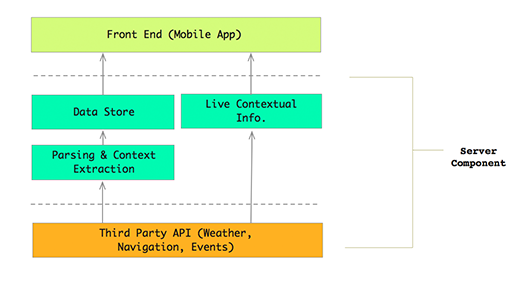
\includegraphics[width=150mm]{AppArch.png}
   \caption [Architecture for the application.]{Architecture for the application.}
 \label{figure:AppArch}
\end{figure}


The API provides a wide range of information depending on the details entered by the user at the time of creation of the event.


\begin{figure}[htbp]
 \centering
 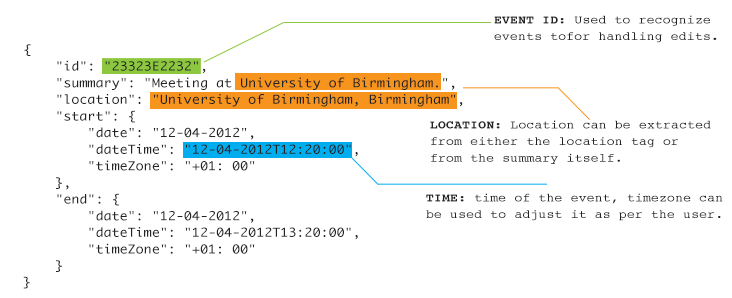
\includegraphics[width=150mm]{DataStructure.png}
   \caption[Structure of an \textit{event}.]{Structure of event from which the information can be extracted and utilised in the application}
 \label{figure:DataStruct}
\end{figure}

The information that is required is limited for our initial development. The first thing we would need is \textit{``id''} which would be required for synchronisation of calendar events between the app and the Google calendar. 
Each event has a title which is entered by the user, this can also contain context information for example location, time etc. However, Google also provides option to enter location information and can be extracted if required. Similarly, start and end date time information along with the timezone can be entered and extracted as well. The architecture will also include a web component. The component stores information about the events, associates it with the user's account and then provide the information in the desired format when queried for.

\section{Application Flow \& Design}

The UI component would be very critical in making the application provide the user a very friendly experience. Overall UI of the application is designed with accordance to Apple's application design guidelines \cite{apple2014hci}. The following are the essential items that were kept in mind while creating a prototype.

\subsection{The Login Interface}

\begin{figure}[htbp]
 \centering
 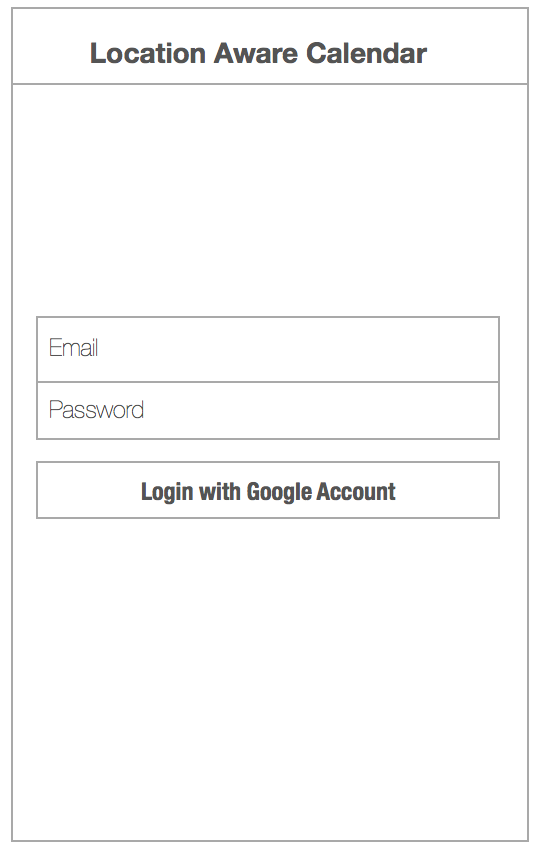
\includegraphics[width=50mm]{LoginScr.png}
   \caption[Login Screen]{Login Screen}
 \label{figure:loginScr}
\end{figure}


The login of the application, is a one time interface that would provide access to the user's calendar. This provides a barrier to protect user information and also allows secure transference of the data. The inferace prototype for the login is shown in the \textit{figure \ref{figure:loginScr}}.

\subsection{The Dashboard}
The dashboard is the primary screen of the application, it showcases the various events from the user's calendar which are relevant to the present day. The present day's agenda is shown in the application with the most recent one being on top with others being swipe-able. The event information is used to extract various other information.

\begin{figure}[htbp]
 \centering
 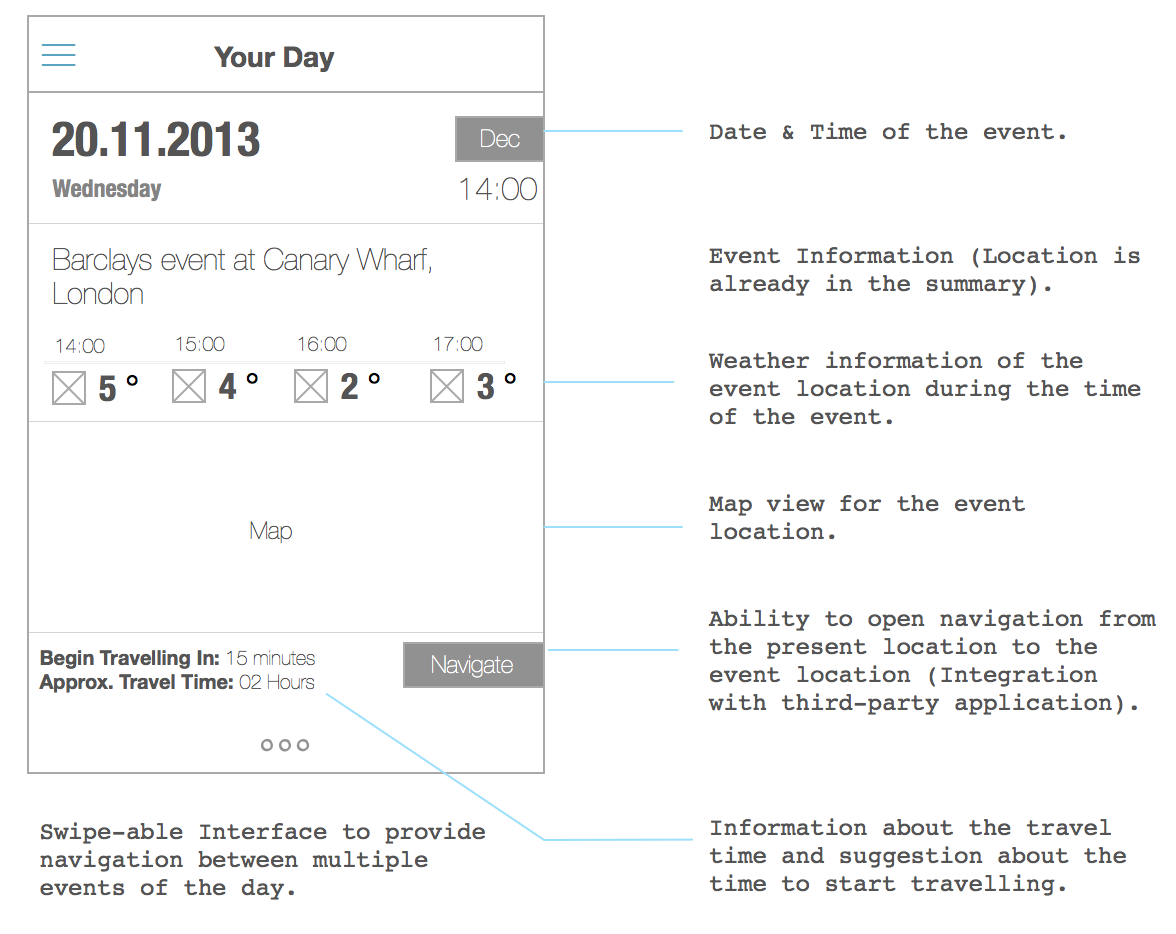
\includegraphics[width=130mm]{DashboardScr.png}
   \caption[Dashboard Sceen]{Dashboard Sceen}
 \label{figure:DashboardScr}
\end{figure}

\begin{itemize}
\item \textit{Weather} - The location of the event is used along with the time of the event to provide weather information about the location during the time period of the event.

\item \textit{Location on the map} - The location of the event is extracted from the event information, either from the title or from the event title. This is then converted into coordinates and would be used to display on the map.

\item \textit{Transit information} - The transit information for the application is calculated based on the user's current location and the event's location. The Google Maps API would be used to extract the information for travel. Based on this the time required for commuting would be extracted and used to show notification before travel.
\end{itemize}
\subsection{Other Features}

\begin{figure}[htbp]
 \centering
 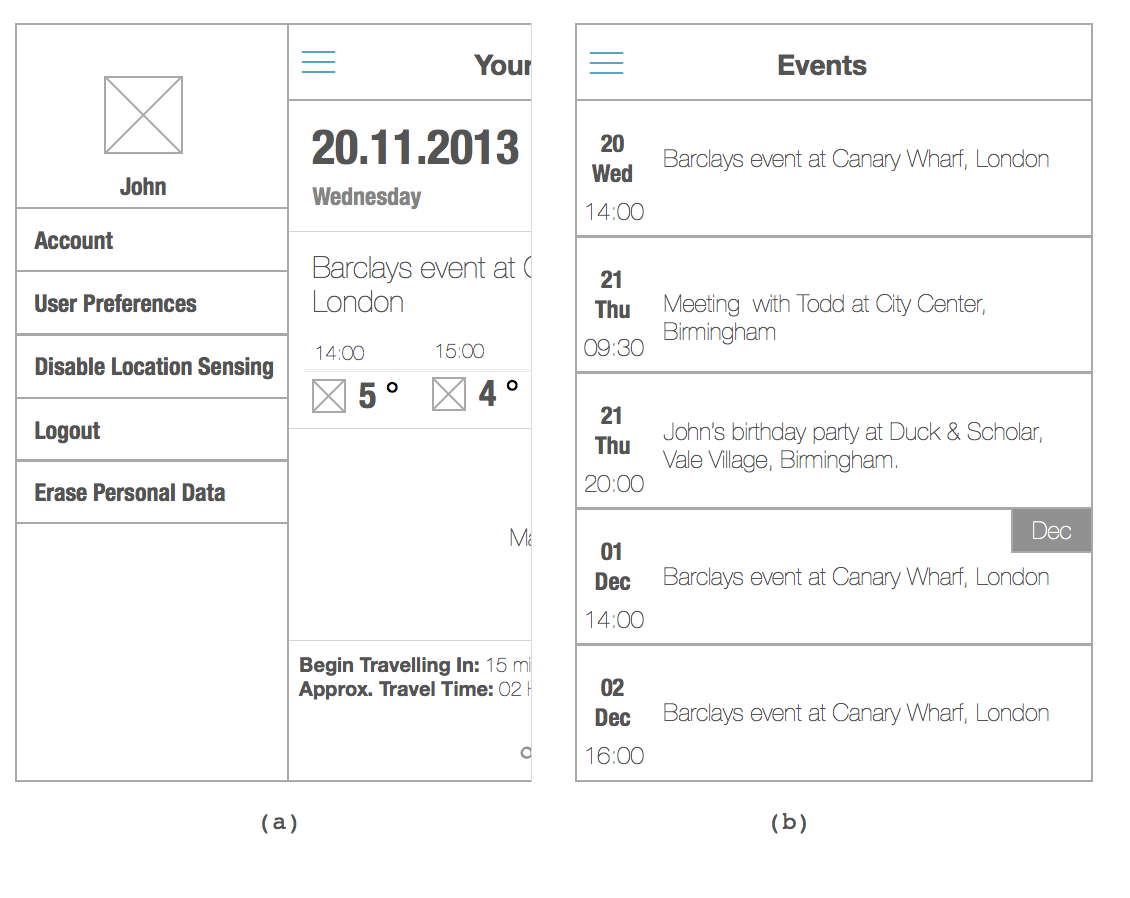
\includegraphics[width=130mm]{AdditionalScr.png}
   \caption[Other Screens]{Other Screens: (a) Settings Panel (b) Event List.}
 \label{fgr:AdditionalScr}
\end{figure}

\begin{itemize}
\item \textit{Event list} - Shows the complete list of the events sorted in a list for the user to view. This would be a generic list for the user to see all the event so that the application can still function as a normal calendar as well.

\item \textit{Settings} - The application would provide various settings for the application's user, this would appear in the side panel and the settings sub-menu option. The following are some of the settings which would be customisable from the application:
\begin{itemize}
\item \textit{Approximate travel time notification} - Time before the application should notify the user about the time required for the travel.
\item \textit{Mode of travel} - The mode of travel the user prefers would be a configurable parameter. This would be used as an input parameter in the transit API methods.
\item \textit{Logout} - The application would provide an option to logout.
\item \textit{Reset/Delete App Data} - The app allows the user to remove all his personal data from the application's database, both in the app locally and on the server.
\end{itemize}
\begin{figure}[htbp]
 \centering
 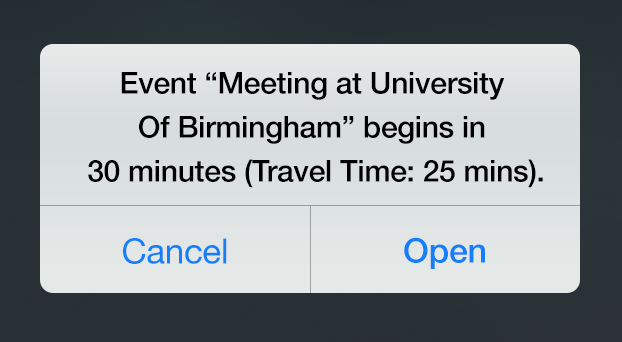
\includegraphics[width=50mm]{EventNotif.png}
   \caption[Begin travel notification.]{A sample begin travel notification presented to notify the user to begin his travel.}
 \label{fgr:EventNotif}
\end{figure}
\item \textit{Notifications} - The notifications would be shown as a means of providing information to the user automatically beforehand. The information about the events would be provided before-hand in order to allow user to take appropriate action.
\end{itemize}

\section{Improvement's Implemented}

The application prototype utilises the various aspects of the research done to provide a possible better approach in the design of location-aware application, especially for mobile devices.
\begin{itemize}
\item \textit{Efficient Location Awareness} - The location awareness is a critical aspect of the application. The awareness would be used to fetch information with a minimal possible power consumption. The app would use the appropriate method to fetch information.

\item \textit{Privacy \& Security} - The information would always be fetched with user's permission. Additionally the server would use secure connection to transfer information. The option to reset the data would allow the user to make sure his information is secure and not stored on the server if he does not wishes to.

\item \textit{HCI Implementation} - The interface designed is based on the interaction guidelines of the platforms, making the application user friendly for the OS's default user.

\item \textit{Invisibility} - The application provides information about event in an invisible way as to not to interfere with the user, the context-awareness of the application reduces the user's need to provide input to a minimum and provide the user information at the time of need, without him specifically asking for it.
\end{itemize}

\chapter{Conclusion \& Future Work}
In this report, we have tried to understand the foundations of location-aware systems and the various aspects that govern its working. The understanding of context and its awareness is the key to designing of location-aware applications that would prove to be useful to the user. However as we have seen context is not just restricted to location, there are various other aspects to it which also prove to be equally essential and work along side location-awareness. With the technological advances where devices are getting smaller and mobile and people's lives are getting more dependent on technology to make it simple, context-awareness has a great role to play. Designers of the systems can no longer consider mobility as an additional aspect in their design of application which previously were targeted for desktop rather they have to design application around the mobility factor and harness its advantages.

The research that has been done here can be further extended by looking into ways in which we can improvise our development strategies to consider mobility as an vital aspect. Additionally, modern platform specific research would be required to look into ways in which context-awareness can be put into use in already existing platforms which are common between the user, making sure the technology that is developed would no longer be restricted to specific set of users but to the general consumer market. As we have seen the success of location-awareness depends on various factors, there are already researches being conducted to improve them, we have provided some suggestions which can prove vital in making the improvements in the modern devices using these techniques, guidelines which can help improve privacy in these application and also the user experience. 

The application prototype that has been showcased here at present is a wireframe and a design idea. It would require improvements as to make it more user-friendly and further refinement with respect to context-awareness can be added in it. The overall prototype would have to go through an initial phase of implementation and a user experience study to make understand any shortcomings and make improvement.

The applications that we have reviewed are just a beginning to the things that can be made possible with location-awareness. The expectation of the modern user has also risen, they are no prepared to even spend to attain information more easily and to make their lives simpler with the help of technology. With devices enabled with location-awareness, this requirement can be met. The user can be provided improved quality of services whether it be finding a place to have their dinner, get through the traffic effectively or make it easier for emergency services to locate them in case of any mishaps. The possibilities are endless and will further grow with advancement of technology.
\bibliographystyle{chicago}
\bibliography{Assigment_III}

%APPENDICES
\appendix
%Mini-project declaration
%\clearpage
\chapter{Mini-Project Declaration}
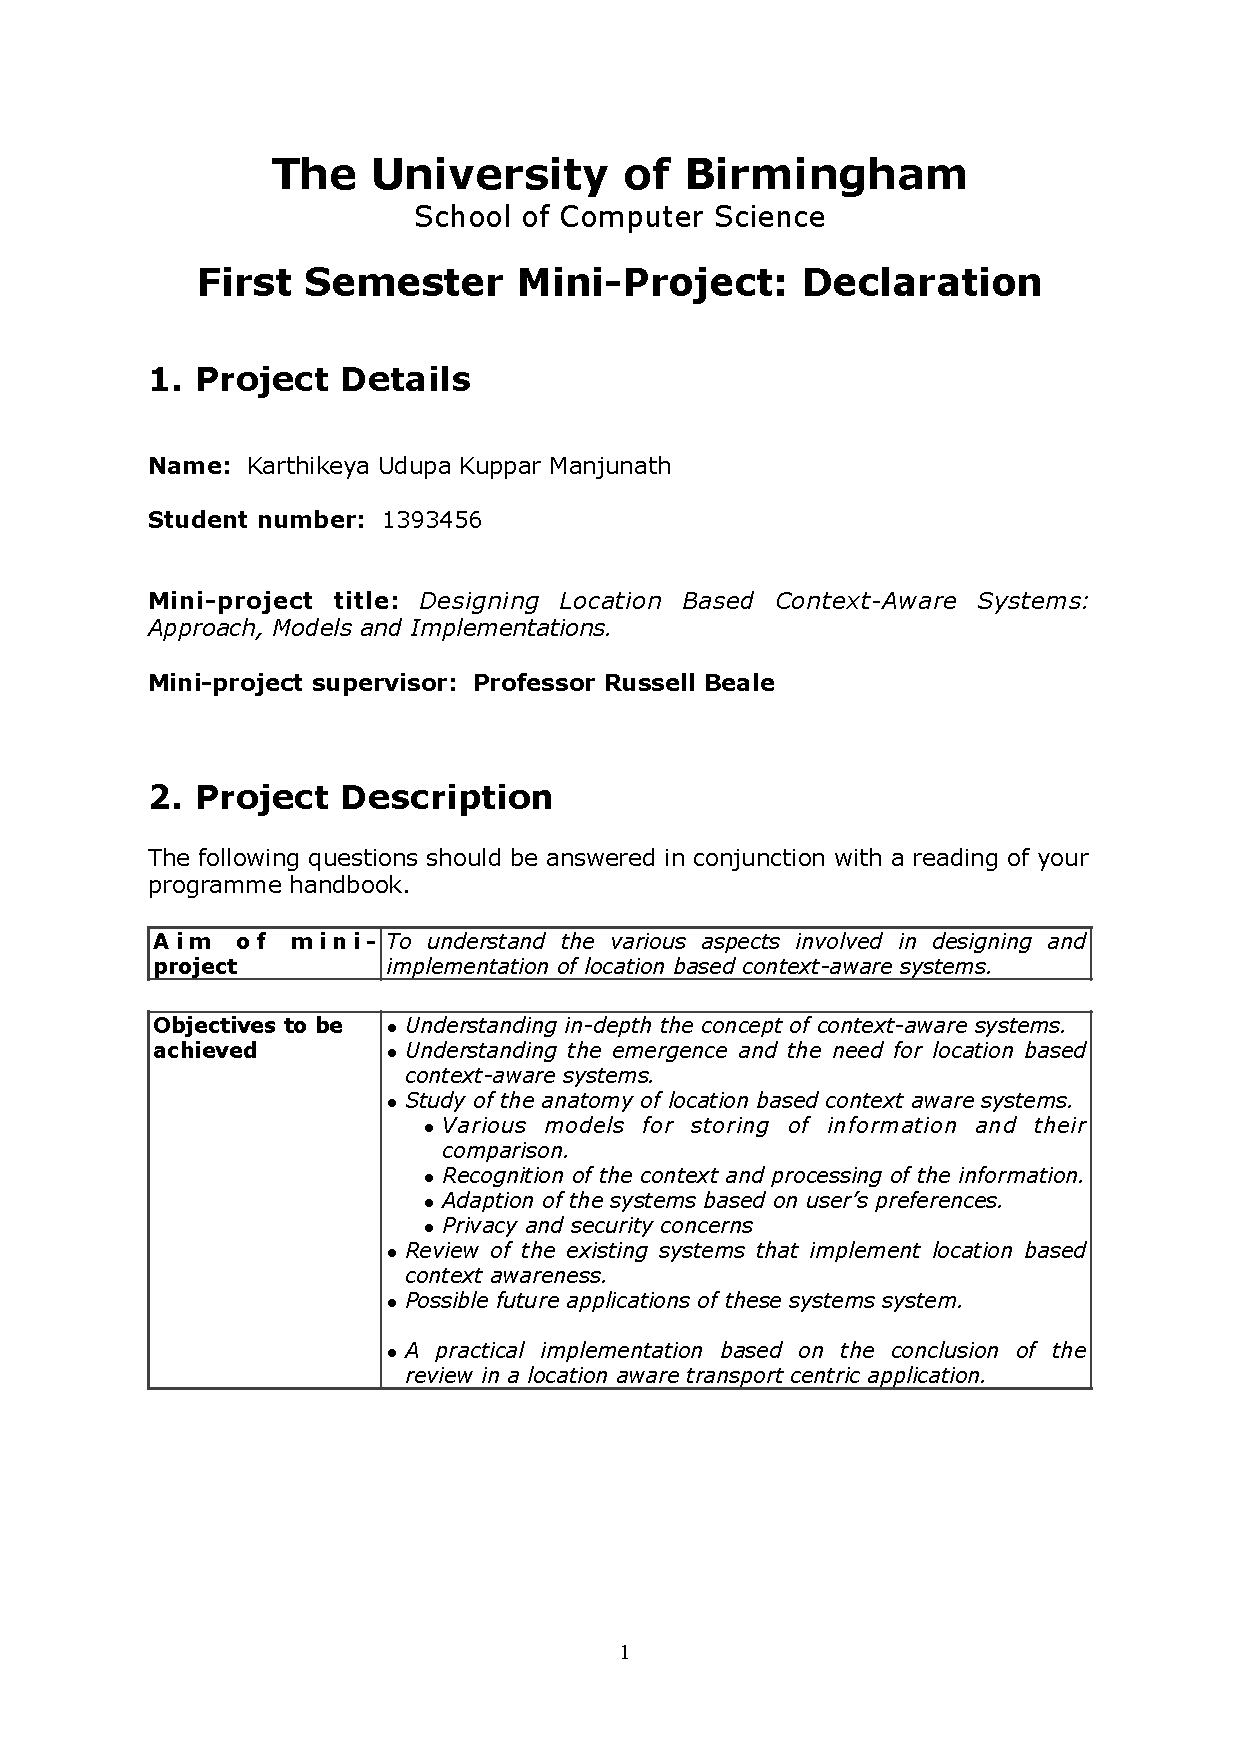
\includepdf[pages={1,2}]{Declaration.pdf}

\chapter{Statement of information search strategy}

The literature search focused on finding information about both location-aware and context-aware systems. More emphasis was given to conference paper, technical reports but certain books were also referred to for a more broader perspective on the topic. The information required was published during the last 2 decades since its still and emerging technology.

The search tools that were used were primarily the \textbf{Engineering Index} and \textbf{Google Scholar}. The subject associates with both practical software implementation and also on the research begin done regarding techniques used to make such technology possible. 

The search statements that were used constituted of various key search terms done over several searches, below are few key statements.
\begin{itemize}
\item Location AND Aware*
\item Context AND Aware*
\item Location AND Model
\end{itemize}

From the results obtained vital literature works were identified. Based on the initial set of literature, citation were searched for. The key authors in the domain were then identified and the work that was done by them and was relevant to the topic were identified.
\end{document}